\documentclass{beamer}

\usetheme[secheader]{Boadilla}
\usecolortheme{crane}
\usepackage[latin1]{inputenc}

\title{Open Source Android Development Tools}
\author{Manfred Moser}
\date{June, 2011}
\institute[2011]{simpligility technologies inc.}

\begin{document}

\begin{frame}
  \titlepage 
\end{frame}

\begin{frame}
  \frametitle{Table of Contents}
  SDK, ADT and beyond
  \setcounter{tocdepth}{1}
  \tableofcontents
\end{frame}


\section{Android Itself}

  \subsection{Components}
    \begin{frame}
      \frametitle{What Components make up Android?}
      \begin{itemize}
        \item<1->Android Proper
        \item<2->AOSP
        \item<3->ADT
      \end{itemize}
    \end{frame}

  \subsection{Android Proper}
    \begin{frame}
    \frametitle{Android Proper - As Found on Your Device}
    \begin{itemize}
      \item<1->Linux
      \item<2->Apache Harmony 
      \item<3->Lots of other open source components
      \item<4->AOSP bits
      \item<5->binary device driver and other blobs 
      \item<6->custom parts from manufacturer and provider
    \end{itemize}
    \end{frame}
  
  \subsection{AOSP}
    \begin{frame}
      \frametitle{Android Open Source Project AOSP}
      \begin{itemize}
        \item<1->open source drops
        \item<2->base for custom roms and such
        \item<3->numerous specific components e.g. Dalvik
        \item<4->various forks from upstream projects
      \end{itemize}
    \end{frame}

  \subsection{ADT}
    \begin{frame}
      \frametitle{Android Development Toolkit ADT}
      \begin{itemize}
        \item<1->open source, fully 
        \item<2->EPL
      \end{itemize}
    \end{frame}

\section{Development Tools}

  \subsection{IDEs}

    \begin{frame}
      \frametitle{Eclipse and ADT and friends}
      
    \end{frame}

    \begin{frame}
      \frametitle{Motorola Motodev Studio for Android}
    \end{frame}

    \begin{frame}
      \frametitle{Jetbrains IntelliJ IDEA CE}
    \end{frame}

    \begin{frame}
      \frametitle{Oracle Netbeans}
    \end{frame}

    \begin{frame}
      \frametitle{Others}
        \begin{itemize}
        \item<1->DroidDraw
        \item<2->EPL
      \end{itemize}
    \end{frame}

  \subsection{Build Tools}

    \begin{frame}
      \frametitle{Maven Android Plugin and Friends}
      \begin{itemize}
       \item Maven Android Plugin \url{http://code.google.com/p/maven-android-plugin/}
       \item Maven Android SDK Deployer \url{https://github.com/mosabua/maven-android-sdk-deployer}
       \item Android4Maven \url{http://sourceforge.net/projects/android4maven/}
       \item M2E Android \url{https://github.com/rgladwell/m2e-android}
       \item AndroidSDKFido \url{https://github.com/joakime/android-sdkfido}
       \item Android RIndirect \url{https://github.com/akquinet/android-rindirect}
      \end{itemize}

    \end{frame}

    \begin{frame}
      \frametitle{Others}
      \begin{itemize}
       \item Gradle Android Plugin \url{https://github.com/jvoegele/gradle-android-plugin}
       \item SBT Android Plugin \url{https://github.com/jberkel/android-plugin}
      \end{itemize}

    \end{frame}

    \begin{frame}
      \frametitle{SBT Android Plugin}
    \end{frame}

  \subsection{Other Languages}
    \begin{frame}
      \frametitle{Other Languages}
      \begin{itemize}
      \item JRuby
      \item Scala
      \item C/C++
      \item CSharp
      \end{itemize}
    \end{frame}

  \subsection{Other Development Tools}

    \begin{frame}
      \frametitle{Other Development Tools}
      \begin{itemize}
        \item<1->Droid at Screen 
        \item<2->dex2jar and others
        \item<3->Android2PO - Converter Android strings to gettext \url{https://github.com/miracle2k/android2po}
      \end{itemize}
    \end{frame}

\section{Development Libraries}


  \subsection{Java Libraries}

    \begin{frame}
      \frametitle{}
      \begin{itemize}
        \item<1->jackson
        \item<2->gson
      \end{itemize}
    \end{frame}

  \subsection{Android Specific Libraries}

    \begin{frame}
      \frametitle{Android Specific Libraries}
      \begin{itemize}
        \item<1->Roboguice \url{http://roboguice.org} 
        \item<2->AndroidAnnotations \url{http://code.google.com/p/androidannotations/}
        \item<3->DroidFu \url{http://github.com/kaeppler/droid-fu}
        \item<4->OpenIntents \url{http://code.google.com/p/openintents/}
        \item<5->AndEngine \url{http://www.andengine.org/}
        \item<6->ksoap2-android \url{http://code.google.com/p/ksoap2-android/}
        \item<7->WSDL2Android \url{https://github.com/kigero/WSDL2Android}
        \item<8->CommonsWare Android Components CWAC \url{https://github.com/commonsguy}  
        \item<9->AndroidAsync \url{https://bitbucket.org/hal/android-async/}  
        \item DroidKit\url{https://github.com/droidkit/droidkit}
\end{itemize}
    \end{frame}

  \subsection{Android UI Libraries}

    \begin{frame}
      \frametitle{UI Libraries}
      \begin{itemize}
       \item<1-> GreenDroid \url{https://github.com/cyrilmottier/GreenDroid}
       \item<2-> ActionBarSherlock \url{http://actionbarsherlock.com/} 
      \end{itemize}

    \end{frame}

    \begin{frame}
      \frametitle{AndroidSherlock}
      \begin{center}
      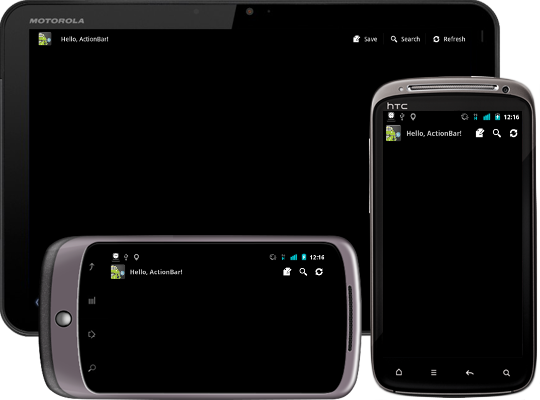
\includegraphics[height=1.0in]{androidsherlock.png}
      \end{center}
    \end{frame}

  \subsection{Android Testing Libraries}

    \begin{frame}
      \frametitle{Android Testing Libraries}
      \begin{itemize}
        \item<1->Robotium \url{http://robotium.org}
        \item<2->Robolectric \url{http://robolectric.org}
        \item<3->Calculon \url{https://github.com/kaeppler/calculon}
        \item<4->Android JUnit Report \url{https://github.com/jsankey/android-junit-report}
      \end{itemize}
    \end{frame}


  \subsection{Others of interest}  

    \begin{frame}
      \frametitle{i-jetty}
      \begin{itemize}
       \item i-jetty \url{http://code.google.com/p/i-jetty/}
      \end{itemize}

    \end{frame}

    \begin{frame}
      \frametitle{web based frameworks}
    \end{frame}

\section{Conclusions}

  \subsection{Android = Java?}
    \begin{frame}
      \frametitle{Is Android Java?}
      \begin{itemize}
      \item<1-> Yes - default application programming language
      \item<2-> Yes - API is Java based
      \item<3-> No - not using a standard compliant Java Virtual Machine Runtime
      \item<4-> No - only using parts of the standard class libraries
      \end{itemize}
    \end{frame}

  \subsection{Android = Open Source?}
    \begin{frame}
      \frametitle{Is Android Open Source?}
      \begin{itemize}
       \item<1-> Yes, in time - AOSP open sourced in drops
       \item<2-> Yes -ADT fully open source
       \item<3-> Yes and no - cooperation with upstream projects
       \item<4-> No - binary blobs for drivers and other parts
      \end{itemize}
    \end{frame}

  \subsection{Android part of Java Community?}
    \begin{frame}
     \frametitle{Android part of the Java Community?}
     \begin{itemize}
      \item<1-> Yes - parts of Android itself
      \item<2-> Yes - tooling around Android
      \item<3-> Yes - lots of libraries and tooling from rest of Java universe
      \item<4-> Yes - lots of people from Java community also in Android community
      \item<5-> Yes - lots of JVM related aspects as well e.g. Scala, JRuby, Processing, Groovy...
      \end{itemize}
    \end{frame}
  
  \subsection{Android part of Open Source Community?}
    \begin{frame}
     \frametitle{Android part of Open Source Community?}
     \begin{itemize}
      \item<1-> Yes - part of Apache Community
      \item<2-> Yes - part of Eclipse Community
      \item<3-> Yes - part of Ruby, Scala, Groovy/Gradle...
      \item<4-> Yes - lots of open source libraries specifically to Android
      \item<5-> Yes - 
      \item<6-> Yes - 
      \item<7-> Yes - 
     \end{itemize}
    \end{frame}

  \subsection{Overall Conclusions}
    \begin{frame}
      \frametitle {Overall conclusion}
      \begin{itemize}
        \item<1-> Despite lots of flaws and kinks
        \item<2-> Android is part of the Java and Open Source communites
        \item<3-> Android is touches a lot more communities 
        \item<4-> Android is a great chance to unify 
      \end{itemize}
    \end{frame}

  \subsection{What can you do?}
    \begin{frame}
      \frametitle{What can you do?}
      \begin{itemize}
        \item<1-> Buy an unlocked/unlockable device
        \item<2-> Use a custom ROM
        \item<3-> Ask for open source drops of AOSP 
        \item<4-> Encourage patches to upstream projects
        \item<5-> Ask for open sourcing of tools
        \item<6-> Contribute and cooperate yourself! 
      \end{itemize}
    \end{frame}
\end{document}